\documentclass[a4paper]{article}

\usepackage{adjustbox}
\usepackage{algorithm}
\usepackage{algorithmic}
\usepackage{amsmath}
\usepackage{amssymb}
\usepackage{amsthm}
\usepackage{amsfonts}
\usepackage{afterpage}
\usepackage{blindtext}
\usepackage[font=footnotesize,labelfont=bf]{caption}
\usepackage{hyperref}
\usepackage[english]{babel}
\usepackage{bbm}
\usepackage{bigints}
\usepackage{bm}
\usepackage{cite}
\usepackage{color}
\usepackage{float}
\usepackage[left=2cm,right=2cm,top=2cm,bottom=2cm]{geometry}
\usepackage{graphicx}
\usepackage[utf8]{inputenc}
\usepackage{mathtools}
\usepackage{mdframed}
\usepackage{pgfplots} 
\usepackage{subfigure}
\usepackage{stmaryrd}
\usepackage{textcomp}
\usepackage{tikz}
\usepackage{url}
\renewcommand{\proofname}{Proof}
\theoremstyle{plain}
\newtheorem{monTheoNumrote}{Théorème}[section] % Environnement numéroté en fonction de la section
\newtheorem*{monTheoNonNumerote}{Théorème}  % Environnement non numéroté
\newtheorem{The}{Theorem}[section]
\newtheorem*{The*}{Theorem}
\newtheorem{Prop}{Proposition}[section]
\newtheorem*{Prop*}{Proposition} 
\newtheorem{Cor}{Corollary}[section]
\newtheorem*{Cor*}{Corollary}
\newtheorem{Conj}{Conjecture}[section]
\newtheorem{Lem}{Lemma}[section]
\renewcommand{\qed}{\unskip\nobreak\quad\qedsymbol}%
\numberwithin{equation}{section} % Numérote les équations section.numéro.
\theoremstyle{definition}
\newtheorem{Def}{Definition}[section]
\newtheorem{Rem}{Remark}[section]
\newtheorem*{Rem*}{Remark}
\newtheorem*{Lem*}{Lemma}
\newtheorem{Que}{Question}
\newcommand{\enstq}[2]{\left\{#1\mathrel{}\middle|\mathrel{}#2\right\}}
\newcommand{\Lp}[2]{L^#1(#2)}
\newcommand{\Sob}[3]{W^{#1,#2}(#3)}
\newcommand{\Rd}[0]{\mathbb{R}^d}
\newcommand{\RN}[0]{\mathbb{R}^N}
\newcommand{\Rn}[0]{\mathbb{R}^n}
\newcommand{\norm}[1]{\left\|#1\right\|}
\newcommand{\sinc}[0]{\textup{sinc}}
\newcommand{\functionDef}[5]{\begin{array}{lllll}
#1 & : & #2 & \longrightarrow & #3 \\
 & & #4 & \longmapsto &\displaystyle #5 \\
\end{array}}
\newcommand{\Theautorefname}{Theorem}
\newcommand{\Propautorefname}{Proposition}
\newcommand{\Corautorefname}{Corollary}
\newcommand{\Lemautorefname}{Lemma}
\newcommand{\Defautorefname}{Definition}
\newcommand{\N}{\mathbb{N}}
\newcommand{\Z}{\mathbb{Z}}
\newcommand{\D}{\mathbb{D}}
\newcommand{\R}{\mathbb{R}}
\newcommand{\A}{\mathcal{A}_{a,b}}
\newcommand{\Crad}{C^\infty_{c,rad}(B)}
\newcommand{\Lrad}{L^2_{rad}(B)}
\newcommand{\Lradab}{L^2_{rad}(\mathcal{A}_{a,b})}
\newcommand{\duality}[2]{\left\langle #1,#2\right\rangle}
\newcommand{\Hrad}{H^1_{rad}(B)}
\newcommand{\Hzrad}{H^1_{0,rad}(B)}
\newcommand{\rmin}{\delta_{\min}}
\newcommand{\rmax}{\delta_{\max}}
\newcommand{\corr}{\gamma}
\newcommand{\question}[1]{\begin{Que} \ 
#1
\end{Que}}
\newcommand{\abs}[1]{\left\lvert #1 \right\rvert}
\newcommand{\CL}[2]{\textup{CL}\left(\enstq{#1}{#2}\right)}
\newcommand{\Script}[1]{`\texttt{#1}`}
\newcommand{\espace}{\text{ }\qquad} 
\newcommand{\loc}{\text{loc}}
\newcommand{\SL}{\textup{SL}\hspace{1.5pt}}
\newcommand{\DL}{\textup{DL}\hspace{1.5pt}}
\newcommand{\fp}{\underset{\varepsilon \to 0}{\textup{f.p.}}}
\newcommand{\scalProd}[2]{\left(#1|#2\right)}
\newcommand{\toDo}[1]{{\color{red}#1}}
\newcommand{\bs}[1]{\boldsymbol{#1}}
\newcommand{\varInRange}[4]{(#1_{#2})_{#3 \leq #2 \leq #4}}
\newcommand{\from}{\colon}
\newcommand{\Cinf}{C^{\infty}}
\newcommand{\isdef}{\mathrel{\mathop:}=}
\newcommand{\defis}{=\mathrel{\mathop:}}

\renewcommand{\algorithmicrequire}{\textbf{Inputs:}}
\renewcommand{\algorithmicensure}{\textbf{Outputs:}}

\pgfplotsset{compat=1.13}

\title{New preconditioners for the Helmholtz integral equation on open cruves}
\author{Fran\c{c}ois Alouges and Martin Averseng\footnote{CMAP, Ecole polytechnique, Route de Saclay, 91128 Palaiseau Cedex.}}
\begin{document}
\maketitle

\begin{abstract}
	We introduce two new preconditioners for the resolution of Helmholtz's integral with Dirichlet or Neumann boundary data, in the form of square roots of local operators. We demonstrate the efficiency of this method on several numerical examples. 
\end{abstract}

\section*{Introduction}

The problem of preconditionning the linear systems coming from the discretization of first kind integral equations
has received considerable attention since two decades roughly. Among the possible strategies are the so-called pseudo-differential preconditionner, whose analysis uses tools from pseudo-differential calculus \cite{christiansen2002preconditioner,Nedelec,Levadoux}. Roughly speaking, if the original problem is written in the abstract way
\begin{equation}
	\mathcal{L}u=f\,,
	\label{eq1}
\end{equation}
the strategy consists in findind a suitable operator $\mathcal{K}$ such
that, when left mulitplying the (\ref{eq1}) by $\mathcal{K}$, one needs to solve
\begin{equation}
	\mathcal{K}\mathcal{L}u=\mathcal{K}f\,.	
\end{equation}
Now if $\mathcal{K}\mathcal{L}$ is a compact perturbation of the identity, the condition number of the discretized underlying linear system is small and independent of the mesh size, enabling the efficient use of iterative methods such as GMRES \cite{gmres}.

Several strategies, depending on the problem to solve have been studied in the literature \cite{} to propose such operators $\mathcal{K}$, that often turn out to be very effective in practice, when numerical applications are considered. However, all the preceding results and theories are limited to smooth domains and very little is known when the integral equation 
is posed on domains with corners (in 2D), wedges or conical points (in 3D). One of the reason might be the fact that pseudo-differential calculus is difficult to generalize on such manifolds, and more problematic, the underlying operators are difficult to analyze on such domains.

Nevertheless, a program similar to those given on smooth manifold was proposed a few years ago \cite{bruno2012second,hiptmair2017closed,jerez2012explicit,hiptmair2014mesh,ramaciotti2017some} who tackled the problem of preconditioning the first or second layer potential
for Laplace or Helmholtz equation in dimension 2 or 3 but for very particular domains: a straight and then curved segment in 2D and a unit disc in 3D. In most of these works, weighted versions of the usual integral operators are introduced, which enjoy better mapping properties than the standard operators. 

Here, we build alternative preconditioners for these weighted operators, using ideas inspired by pseudo-differential theory. These preconditioners are in the form of the square root of local operators, in close analogy to \cite{antoine2007generalized}. 
	
The paper is organized as follows: in the first section, we introduce the notations and the usual boundary integral operators on an open curve. In the second section, we treat the case of the Laplace equation, where it is possible to derive explicit inverses of the weighted layer potentials in terms of square roots of local operators. We then generalize our results to non-zero frequency and non-flat arc in the third section. In the last section, we show the efficiency of this approach on several numerical examples. 

\section{The scattering problem outside an open curve}

Let $\Gamma$ be a smooth non-intersecting open curve, and let $k \geq 0$ the wave number. We seek a solution of the problem
\begin{equation}
	-\Delta u - k^2 u = 0,  \text{ in } \R^2 \setminus \Gamma
	\label{Helmholtz}
\end{equation}
when one considers furthermore
\begin{itemize}
	\item Dirichlet or Neumann boundary conditions, namely
	\begin{equation}
	u = u_D, \text{ on } \Gamma
	\label{Dirichlet}
	\end{equation}
	or
	\begin{equation}
	\dfrac{\partial u}{\partial n} = u_N  \text{ on } \Gamma 
	\label{Neumann}
	\end{equation}
	respectively.
	\item Suitable decay at infinity, given by the Sommerfeld condition
	\begin{equation}
	\dfrac{\partial u}{\partial r} - iku = o\left(\frac{1}{\sqrt{r}}\right)
	\label{Sommerfeld}
	\end{equation}
	with $r=|x|$ for $x\in \mathbb{R}^2$.
\end{itemize}
In the preceding equation $n$ stands for a smooth unit normal vector of $\Gamma$. 

\noindent Existence and uniqueness of solutions to the previous problems are guaranteed by the following theorem.
\begin{The}
	(see e.g. \cite{stephan1984augmented,wendland1990hypersingular,monch1996numerical}) Assume $u_D \in H^{1/2}(\Gamma)$, and $u_N \in H^{-1/2}(\Gamma)$. Then problems (\ref{Helmholtz},\ref{Dirichlet},\ref{Sommerfeld}) and (\ref{Helmholtz},\ref{Neumann},\ref{Sommerfeld}) both possess a unique solution $u \in H^1_\textup{loc}(\R^2 \setminus \Gamma)$, which is of class $C^{\infty}$ outside $\Gamma$. Near the edges of the screen $\Gamma$ $\lambda$ is unbounded:
	\[\lambda(x) = O\left(\frac{1}{\sqrt{d(x,\partial \Gamma)}}\right).\]
	Near an edge of the arc, $\mu$ is locally given by
	\[\mu(x) = C\sqrt{d(x,\partial \Gamma)} + \psi.\]
	where $\psi \in \tilde{H}^{3/2}(\Gamma)$ and $C$.
\end{The}
\noindent For the definition of Sobolev spaces on smooth open curves, we follow
\cite{mclean2000strongly} by considering any smooth closed curve $\tilde{\Gamma}$ containing $\Gamma$, and defining 
\[H^s(\Gamma) = \enstq{U_{|\Gamma}}{ U \in H^s(\tilde{\Gamma}) }.\]
Obviously, this definition does not depend on the particular choice of the closed curve $\tilde{\Gamma}$ containing $\Gamma$. Moreover,
\[\tilde{H}^s(\Gamma) = \enstq{u \in H^s(\Gamma)}{\tilde{u} \in H^s(\tilde{\Gamma})}\]
where $\tilde{u}$ denotes the extension by zero of $u$ on $\tilde{\Gamma}$.

\paragraph{Single-layer potential}  
The single-layer potential is defined by
\begin{equation}
	\mathcal{S}_k\lambda(x) = \int_{\Gamma}G_k(x-y)\lambda(y)d\sigma(y)
	\label{defSk}
\end{equation}
	where $G_k$ is the Green's function
\begin{equation}
	\left\{
	\begin{aligned}
		G_0(z) &= -\dfrac{1}{2\pi} \ln \abs{z}, && \text{ if } k= 0,\\
		G_k(z) &= \frac{i}{4}H_0(k|z|), && \text{ if } k > 0,
	\end{aligned} 
	\right.
\end{equation} 
for $x\in \mathbb{R}^2\setminus \Gamma$, and where $H_0$ is the Hankel function of the first kind. 
The solution $u$ of the Dirichlet problem can be computed from (\ref{Helmholtz},\ref{Dirichlet},\ref{Sommerfeld}) as
\begin{equation}
	u = \mathcal{S}_k \lambda
\end{equation}
where $\lambda \in \tilde{H}^{-1/2}(\Gamma)$ is the unique solution to 
\begin{equation}
	S_k \lambda = u_D\,.
	\label{Sklambda}
\end{equation}
Here, $S_k \isdef \gamma \mathcal{S}_k$ where $\gamma$ is the trace operator on $\Gamma$. The operator $S_k$ maps continuously $\tilde{H}^{-1/2}(\Gamma)$ to $H^{1/2}(\Gamma)$.

\paragraph{Double-layer and hypersingular potentials}
Similarly, we introduce the double layer potential $\mathcal{D}_k$ by 
\[\mathcal{D}_k \mu(x) = \int_{\Gamma} n(y) \cdot \nabla G_k(x-y) \mu(y) d\sigma(y).\]
for any smooth function $\mu$ defined on $\gamma$.
The normal derivative of $\mathcal{D}_k\mu$ is continuous across $\Gamma$, allowing us to define the hypersingular operator $N_k = \partial_n \mathcal{D}_k$. This operator admits the representation for $x\in \Gamma$
\begin{equation}
	N_k \mu = \lim_{\varepsilon \to 0^+} \int_{\Gamma} n(y) \cdot \nabla G(x + \varepsilon n(x) - y) \mu(y) d\sigma(y).
	\label{defNk}
\end{equation}
The kernel of this operator has a non-integrable singularity, but numerical calculations are made possible by the following formula, valid for smooth functions $\mu$ and $\nu$ that vanish at the extremities of $\Gamma$: 
\begin{equation}
	\begin{split}
		\duality{N_k \mu}{\nu} = &\int_{\Gamma\times \Gamma} G_k(x-y) \mu'(x) \nu'(y)\\
		&- k^2 G_k(x,y) \mu(x) \nu(y) n(x) \cdot n(y) d\sigma(x) d\sigma(y)\,.
	\end{split}
	\label{NkenfonctiondeSk}
\end{equation}

It is also known that $N_k$ maps $\tilde{H}^{1/2}(\Gamma)$ to $H^{-1/2}(\Gamma)$ continuously, and that the solution $u$ to the Neumann problem (\ref{Helmholtz},\ref{Neumann},\ref{Sommerfeld}) can be written as
\begin{equation}
	u = \mathcal{D}_k \mu
\end{equation}
where $\mu \in \tilde{H}^{1/2}(\Gamma)$ solves
\begin{equation}
	N_k \mu = u_N\,.
	\label{Nkmu}
\end{equation}  
	
\section{Laplace equation on a flat segment}

In this section, we restrict our attention to the case where $\Gamma$ is the open segment $(-1,1) \times \{0\}$, and the wavenumber $k=0$. We study the properties of the equations 
\[S\lambda = -u_D\]
and 
\[N\mu = u_N\]
This problem has been considered thoroughly, both
in terms of analytical and numerical properties in the literature (see for instance \cite{jiang2004second,bruno2012second}), and it turns out that the Chebyshev polynomials of first and second kind play a very important role. However, to the best of our knowledge, the natural inverses in terms of square roots of local operators have remained unexploited. 

\subsection{Analytical setting}

We first introduce a basic analytic setting to analyze the previous two integral equations.	We introduce the Chebyshev polynomials of first and second kinds, respectively given by 
\[T_n(x) = \cos(n \arccos(x)),\]
and 
\[U_n(x) = \dfrac{\sin((n+1) \arccos(x))}{\sqrt{1 - x^2}}\,.\]
Let $\omega$ the operator $u(x) \mapsto \omega(x)u(x)$ with $\omega(x) = \sqrt{1 - x^2}$. Moreover, let $\partial_x$ the derivation operator. The Chebyshev polynomials satisfy
the ordinary differential equations

\begin{eqnarray*}
	(1-x^2)T_n'' -xT_n' +n^2T_n =0\,\mbox{ and }(1-x^2)U_n'' -3xU_n' +n(n+2)U_n =0
\end{eqnarray*}
which can be rewritten under the form
\begin{eqnarray}
	(\omega\partial_x)^2 T_n &=& -n^2T_n\,, \label{cheb1}\\
	(\partial_x\omega)^2 U_n &=& -(n+1)^2U_n\, .\label{cheb2}
\end{eqnarray}
(Notice that by $(\partial_x\omega) f$ we mean $(\omega f)'$.) Both $T_n$ and $U_n$ are polynomials of degree $n$, and form orthogonal families respectively of the Hilbert spaces 
$$L^2_{\frac{1}{\omega}} \isdef \enstq{u \in L^1_\textup{loc}(-1,1)} {\int_{-1}^{1} \dfrac{f^2(x)}{\sqrt{1 - x^2} }dx< + \infty}$$
and 
$$L^2_{\omega} \isdef \enstq{u \in L^1_\textup{loc}(-1,1)} {\int_{-1}^{1} {f^2(x)}{\sqrt{1 - x^2} }dx< + \infty}.$$
We denote by $\duality{\cdot}{\cdot}_\frac{1}{\omega}$ and $\duality{\cdot}{\cdot}_\omega$ the inner products in $L^2_{\frac{1}{\omega}}$ and $L^2_{\omega}$ respectively.
The Chebyshev polynomials satisfy
\begin{equation}
	\int_{-1}^1  \dfrac{T_n(x)T_m(x)}{\sqrt{1 - x^2} }dx = \left\{
	\begin{array}{l}
	0 \mbox{ if } n\ne m\\
	\pi \mbox{ if } m=n=0\\
	\pi/2 \mbox{ otherwise}
	\end{array} 
	\right.
\end{equation}
	and
\begin{equation}
	\int_{-1}^1  U_n(x)U_m(x)\sqrt{1 - x^2} dx = \left\{
	\begin{array}{l}
	0 \mbox{ if } n\ne m\\
	\pi/2 \mbox{ otherwise}
	\end{array} 
	\right.
\end{equation}
which provides us with the so-called Fourier-Chebyshev decomposition. Any
$u\in L^2_{\frac{1}{\omega}}$ can be decomposed through the first kind Chebyshev series 
\begin{equation}
	u(x) = \sum_{n=0}^{+\infty} \hat{u}_n T_n(x)
	\label{FCseries}
\end{equation}
where the Fourier-Chebyshev coefficients $\hat{u}_n$ are given by 
\[ \hat{u}_n \isdef \begin{cases}
\dfrac{2}{\pi}\displaystyle\int_{-1}^{1} \dfrac{u(x) T_n(x)}{\sqrt{1-x^2}}dx & \text{ if } n \neq 0\,,\\
\dfrac{1}{\pi}\displaystyle\int_{-1}^{1} \dfrac{u(x)}{\sqrt{1-x^2}}dx & \text{ otherwise,}\\
\end{cases}\]
and satisfy the Parseval equality
\[ \int_{-1}^{1} \frac{u^2(x)}{\sqrt{1-x^2}} dx =  \frac{\pi \hat{u}_0^2}{2} + \pi\sum_{n=1}^{+\infty}\hat{u}_n^2\,.\]
When $u$ is furthermore a smooth function, the series \eqref{FCseries} converges uniformly to $u$. Similarly, any 
function $v\in L^2_{\omega}$ can be decomposed along the $U_n$ as
\[ v(x) = \sum_{n=0}^{+\infty} \check{v}_n U_n(x)\]
where the coefficients $\check{v}_n$ are given by 
\[ \check{v}_n \isdef 
\dfrac{2}{\pi}\displaystyle\int_{-1}^{1} v(x) U_n(x)\sqrt{1-x^2}dx  \]
with the Parseval identity
\[ \int_{-1}^{1} v^2(x)\sqrt{1-x^2} dx =  \frac{\pi}{2} \sum_{n=0}^{+\infty}\check{v}_n^2\,.\]
The preceding analysis can be generalized to define Sobolev-like spaces. 
\begin{Def}
	For all $s \geq 0$, we may define 
	\[T^s = \enstq{ u \in L^2_\frac{1}{\omega}}{ \sum_{n=0}^{+\infty}(1+n^2)^s \hat{u}_n^2 < + \infty}.\]
	This is a Hilbert space for the scalar product
	\[\duality{u}{v}_{T^s} = \frac{\pi}{2}\hat{u}_0 \hat{v}_0 + \pi\sum_{n=1}^{+\infty}(1+n^2)^s\hat{u}_n \hat{v}_n.\]
	We also define a semi-norm 
	\[\abs{u}_{T^s} \isdef \sum_{n = 1}^{+ \infty}n^{2s} \abs{\hat{u}_n}^2.\]
	We denote by $T^{\infty}$ the Fr\'echet space $T^{\infty} \isdef \displaystyle\cap_{s \in \R} T^s$, and by $T^{-\infty}$ the set of continuous linear forms on $T^{\infty}$. For $l \in T^{-\infty}$, we note $\hat{l}_n = l(T_n)$, so that for $u \in T^{\infty}$, 
	\[l(u) = \frac{\pi}{2}\hat{l}_0 \hat{u}_0 + \pi \sum_{n=1}^{+\infty} \hat{l}_n \hat{u}_n\,.\] 
		
	We choose to identify the dual of $L^2_\frac{1}{\omega}$ to itself using the previous bilinear form.  With this identification, any element of $T^s$ with $s \geq 0$ can also be seen as an element of $T^{-\infty}$.  
	Furthermore, the space $T^{-s}$ can be defined for all $s \geq 0$ as
	\[T^{-s} = \enstq{ u \in T^{-\infty}}{ \sum_{n=0}^{+\infty}{(1 + n^2)^{-s} \hat{u}_n^2} < \infty}.\]
	Using the former identification $T^{-s}$ becomes the dual of $T^s$. 
	For $s < t$, the inclusion $T^s \subset T^t$ is compact.
\end{Def}

\noindent In a similar fashion, we define the following spaces:
\begin{Def}
	For all $s \geq 0$, we set
	\[U^s = \enstq{u \in L^2_\omega}{ \sum_{n=0}^{+\infty} (1 + n^2)^s\check{u}_n^2}.\]
	We extend as before the definition to negative indices by setting $U^{-s}$ to be the dual of $U^s$ for $s\geq 0$, this time with respect to the duality $\duality{\cdot}{\cdot}_\omega$. 
\end{Def}
The spaces $T^n$ correspond, up to a variable change, to the spaces $H^n_e$ defined in \cite{bruno2012second,atkinson1991numerical,yan1988integral,yan1990cosine} among other works, that is, the restriction of the usual Sobolev space $H^n$ to even periodic functions. A function $u$ is in $T^s$ if and only if there exists $\tilde{u} \in H^s_e$ such that $u(x) = \tilde{u}(\arccos(x))$. For the spaces $U^s$, the identification is as follows: a function $u$ lies in $U^s$ if and only if it is of the form \[ u(x) = \frac{1}{\omega(x)} v(\arccos(x)).\]
where $v$ is an odd function in $H^s$. For $s = \pm \frac{1}{2}$, those spaces have been analyzed (with different notations) in \cite{jerez2012explicit}, with the following identifications:
\begin{equation}
	\label{lemJerez1}
	T^{-1/2} = \frac{1}{\omega} \tilde{H}^{-1/2}(-1,1), \quad T^{1/2} = H^{1/2}(-1,1)
\end{equation}
\begin{equation}
	\label{lemJerez2}
	U^{-1/2} = H^{-1/2}(-1,1), \quad U^{1/2} = \omega \tilde{H}^{1/2}(-1,1)
\end{equation}
\noindent The polynomials $T_n$ and $U_n$ are connected by the following formulas:
\begin{equation}
\label{TnAsUn}
\forall n \geq 2, \quad T_n(x) = \frac{1}{2}\left(U_n - U_{n-2}\right),
\end{equation}
\begin{equation}
\label{UnAsTn}
\forall n \in \N, \quad U_{2n} = 2\sum_{j = 0}^n T_{2j} - 1, \quad U_{2n+1} = 2\sum_{j=0}^n T_{2j+1}.
\end{equation}

\begin{Lem}
	\label{inclusionsTsUs}
	For all real $s$, $T^s \subset U^s$ and for all $s > 1/2$, $U^s \subset T^{s-1}$.
\end{Lem}
\begin{proof}
	The first property is immediate from \eqref{TnAsUn}. 
	When $u \in U^{s}$ for $s > 1/2$, the series $\sum \abs{\check{u}_n}$ is converging, allowing to identify $u$ to a function in $T^{-\infty}$, with, in view of \eqref{UnAsTn}, 
	\[\hat{u}_{0} = \sum_{n=0}^{+ \infty} \check{u}_{2n}, \quad  \hat{u}_j = 2\sum_{n=0}^{+\infty} \check{u}_{j + 2n} \textup{ for } j \geq 1.\]
	Since $u \in U^s$, $(1+n^2)^{s/2} \abs{\check{u}}$ is in $l^2$ and by continuity of the adjoint of the Cesàro operator in $l^2$, the sequence $r_n \isdef \left( \sum_{k=n}^{+ \infty} (1+k^2)^{\frac{s-1}{2}} \abs{\check{u}_k}\right)_n$ is in $l^2$. But
	\begin{eqnarray*}
		\norm{u}_{T^{s-1}}^2 &=& \sum_{n=0}^{+ \infty} (1 + n^2)^{s-1} \abs{\hat{u}_n}^2\\ 
		&\leq& 4\sum_{n=0}^{+\infty}(1+n^2)^{s-1} \left(\sum_{k=n}^{+\infty} \abs{\check{u}_k}\right)^2 \\
		&\leq& 4\sum_{n=0}^{+ \infty}\left(\sum_{k=n}^{+\infty}(1+k^2)^{\frac{s-1}{2}} \abs{\check{u}_k})\right)^2.\\
		&=& 4\norm{r_n}^2_{l^2}.
	\end{eqnarray*}	
\end{proof}
\noindent One immediate consequence is that $T^{\infty} = U^{\infty}$.  Moreover, we have the following result:
\begin{Lem}
	\[T^{\infty} = C^{\infty}([-1,1])\,.\]
	\label{LemTinfCinf}
\end{Lem}
\begin{proof}
	If $u \in C^{\infty}([-1,1])$, then we can obtain by induction using integration by parts and \eqref{cheb1}, that for any $k \in \N$
	\[\hat{u}_n = \frac{(-1)^k}{n^{2k}} \int_{-1}^{1} \dfrac{(\omega\partial_x)^{2k} u(x) T_n(x)}{\omega(x)}dx.\]
	Noting that $(\omega \partial_x)^2 = (1-x^2)\partial_x^2 - x \partial_ x$, this proves that $C^{\infty}([-1,1]) \subset T^{\infty}$. 
	
	To prove the converse inclusion, first notice that, by normal convergence of the series, $T^{\infty} \subset C^0([-1,1]) $. Now, let $u \in T^{\infty}$, it suffices to show that $u' \in T^{\infty}$ and apply an induction argument. Applying term by term differentiation, we obtain
	\[u'(x) = \sum_{n=1}^{+\infty} n u_n U_{n-1}(x).\] 
	Therefore, $u'$ is in $U^{\infty} = T^{\infty}$. 
\end{proof}

\subsection{Single layer equation}

In the case of Dirichlet condition, we seek a solution to the equation $S\lambda = g$, with $\lambda \in \tilde{H}^{-1/2}(\Gamma)$, that is
\begin{equation}
-\frac{1}{2\pi}\int_{-1}^{1} \log|x-y| \lambda(y) = -g(x), \quad \forall x\in (-1,1)\,.\label{Slambda}
\end{equation} 

This equation is sometimes called ``Symm's integral equation'' and its resolution has received a lot of attention in the 1990's. Numerical methods, using both collocation and Galerkin have been presented and analyzed \cite{atkinson1991numerical,yan1988integral,yan1990cosine,sloan1992collocation,yan1989mesh}. 

%The solution is connected to the exterior Dirichlet problem for the Laplace operator, but attention must be paid when the solution $\lambda$ obtained does not satisfy $\duality{1}{\lambda}_\Gamma = 0$: in this case, $\textup{SL}\lambda$ is not a bounded solution of the Dirichlet problem. See \cite{atkinson1991numerical} for a link with the logarithmic capacity of the line and how we recover the bounded solution from the solution of \eqref{Slambda}.

Our analysis lies on the following formula. For a proof, see for example \cite{mason2002chebyshev} Theorem 9.2. Note that this is also the main ingredient in several connected works, such as \cite{jiang2004second} and \cite{bruno2012second}.

\begin{Lem}
	\[ -\frac{1}{2\pi}\int_{-1}^{1} \frac{\ln|x-y|}{\sqrt{1 - y^2}}T_n(y)dy = s_n T_n(x)\]
	where
	\[s_n = \begin{cases}
	\dfrac{\ln(2)}{2} & \text{if } n=0\\
	\dfrac{1}{2n} & \text{otherwise}.
	\end{cases}\]
	\label{STn}
\end{Lem}

Using the decomposition of $g$ and of the logarithmic kernel on the basis $T_n$, we see that the solution $\lambda$ to equation \eqref{Slambda} admits the following expansion 
\begin{equation}
\lambda(x) = \frac{1}{\sqrt{1-x^2}}\sum_{n=0}^{+ \infty} \frac{\hat{g}_n}{s_n} T_n(x).
\label{expansionLambda}
\end{equation}
We deduce the following well-known fact:
\begin{Cor}
	\label{CorSingularity}
	If the data $g$ is in $C^{\infty}([-1,1])$, the solution $\lambda$ to the equation 
	\[S\lambda = g\]
	is of the form 
	\[\lambda = \dfrac{\alpha}{\sqrt{1-x^2}}\]
	with $\alpha \in C^{\infty}([-1,1])$.  
	\begin{proof}
		Let $\alpha = \sqrt{1 - x^2}\lambda$ where $\lambda$ is the solution of $S\lambda = g$.  By \autoref{LemTinfCinf}, if $g \in C^{\infty}([-1,1])$, then $g \in T^{\infty}$, and by equation \eqref{expansionLambda}, 
		\[ \hat{\alpha}_n = \frac{\hat{g}_n}{s_n},\]
		so $\alpha$ also  belongs to $T^{\infty} = C^{\infty}([-1,1])$. 
	\end{proof}
\end{Cor}
\noindent Following \cite{bruno2012second}, we introduce the weighted single layer operator as the operator that appeared in \autoref{STn}.
\begin{Def}
	Let $S_\omega$ be the weighted single layer operator defined by
	\[\opFromTo{S_\omega}{\alpha \in \Cinf([-1,1])}{-\dfrac{1}{2\pi}}{\int_{-1}^1\dfrac{\ln|x-y|}{\omega(y)} \alpha(y)dy}\]
\end{Def}
\noindent To obtain the solution of \eqref{Slambda}, we thus solve 
\begin{equation}
	S_\omega \alpha = -u_D,
	\label{Somegaalpha}
\end{equation}
and let $\lambda = \frac{\alpha}{\omega}$, which indeed belongs in $\tilde{H}^{-1/2}$ by the identifications \eqref{lemJerez1}. From the previous considerations, the inverse for $S_\omega$ can be derived by building an operator $R$ such that $RT_n = \frac{1}{s_n}T_n$. It turns out that such an operator $R$ has been characterized in \cite{jerez2012explicit,urzua2014optimal}, through explicit variational forms in closed forms. A similar method is also employed in the recent paper \cite{hiptmair2017closed} in $\R^3$ for the case of the unit disk. We just state here the following formal decomposition:
\[\dfrac{d^2}{dxdy}\log\frac{M(x,y)}{|x-y|^2} = \frac{-1+xy}{2|x-y|^2} = \sum_{n=1}^{+ \infty} n T_n(x)T_n(y)\]
with 
$M(x,y) = \frac{1}{2}\left((y-x)^2 + (\omega(x) + \omega(y))^2\right) $.

Here, we give an alternative form for the operator $R$, that we will then generalize for a non-zero frequency. 
\noindent Recall that the operator $(\omega\partial_x)^2$ is defined by \[\opFromTo{(\omega\partial_x)^2}{\alpha \in \Cinf([-1,1])}{(1-x^2)\alpha''(x) - x \alpha'(x)}.\]
with $(\omega \partial_x)^2T_n = -n^2 T_n$. Therefore, for $n \neq 0$, since $s_n = \frac{1}{2n}$, we have $(\omega \partial_x)^2 (S_\omega)^2 T_n = 4 T_n$. Thus, we must simply deal with the case $n=0$. For this, we consider a third operator $\pi_{0}$ as the $L^2_{1/\omega}$ orthogonal projector on $T_0$. Namely 
\[\pi_0 \alpha(x)  = \frac{1}{\pi} \int_{-1}^{1}\frac{\alpha(y)}{\omega(y)}dy\,.\] 
Of course, $\pi_0$ is continuous from $T^s$ to $T^{\infty}$ for any $s$. We then have
\begin{The}
	\label{TheSdx2S}
	For any $s$, the operator $-(\omega\partial_x)^2 + \frac{1}{\ln(2)^2} \pi_0 $ is bicontinuous from $T^{s+2}$ to $T^s$ and
	\begin{equation*}
		S_{\omega}^2 = \frac{1}{4}\left(-(\omega\partial_x)^2 + \frac{1}{\ln(2)^2} \pi_0 \right)^{-1}\,.
	\end{equation*}
\end{The}
\noindent The inverse of $S_\omega$ can thus be equivalently expressed as 
\[S_{\omega}^{-1} = 2\sqrt{-(\omega \partial_x)^2 + \frac{1}{\ln(2)^2}\pi_0}\,\]
where the square root of the operator is defined using standard spectral theory. 

The previous considerations show that $\sqrt{-(\omega \partial_x)^2}$ and $S_\omega$ can be thought as inverse operators (modulo constant terms) and that, at the very least, $\sqrt{-(\omega \partial_x)^2}$ can be used as a preconditioner for $S_\omega$. Indeed, $2\sqrt{-(\omega \partial_x)^2}S_\omega$ is a compact perturbation of identity. 

In \autoref{TableNitTimeLaplaceDirichlet}, we report the number of iterations for the numerical resolution of Equation \eqref{Somegaalpha} by the method detailed in \autoref{sec:numerMeth} without preconditioner, and with a preconditioner given by $M^{-1} \left[B \right] M^{-1}$ where $M$ is the mass matrix and $\left[ B \right]$ is the Galerkin matrix of the operator $\sqrt{ -(\omega \partial_x)^2 + \frac{1}{\ln(2)^2} \pi_0}$. The right hand side in \eqref{Somegaalpha} is chosen as $u_D(x) = (x^2 + 0.001)^{-1/2}, x \in (-1,1)$.

\begin{table}[H]
	\begin{center}
		\begin{tabular}{||m{4em}|m{4em}|m{4em}|m{4em}| m{4em}||} 
			\hline
			\multicolumn{1}{||c|}{ }&
			\multicolumn{2}{c|}{with Prec.}&\multicolumn{2}{c||}{without Prec.}\\
			\hline
			$N$ & $n_{it}$& t(s) & $n_{it}$ & t(s)\\
			\hline\hline
			50 & 7 & 0.11 & 35 & 0.21\\
			\hline
			200 & 7 & 0.14 & 53 & 0.55\\
			\hline
			800 & 7 & 0.29 & 76 & 2.0 \\
			\hline
			3200 & 7 & 0.95 & 107 & 9.5\\
			\hline
		\end{tabular}
		\caption{Number of iteration and time needed for the numerical resolution of \eqref{Somegaalpha} using Galerkin finite elements with and without preconditioner.}
		\label{TableNitTimeLaplaceDirichlet}
	\end{center}
\end{table}
\begin{figure}[H]
	\centering
	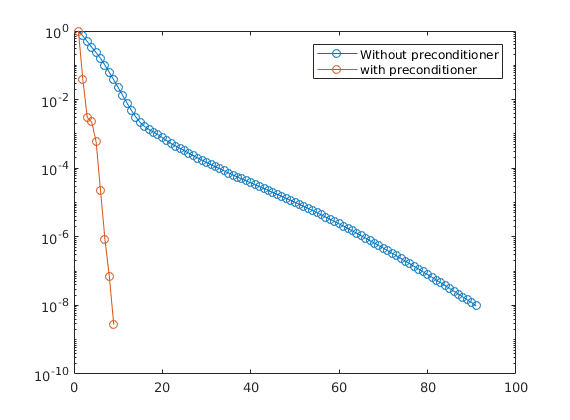
\includegraphics[scale=0.7]{../figs/PrecondDirichletLaplaceSeg.png}
	\caption{Number of iteration in the resolution of the single layer integral equation with a mesh of size $N = 1600$.}
	\label{FigureNitLaplaceDirichlet}
\end{figure}

\subsection{Hypersingular equation} 

We now turn our attention to the equation 
\begin{equation}
N\mu = g
\label{Nmu}
\end{equation} 
\noindent Similarly to the previous section, we consider the weighted version of the hypersingular operator $N_\omega \isdef N \omega$ defined by
\[N_\omega \mu = \lim_{\varepsilon\to 0}\int_{-1}^{1} n(y)\cdot\nabla G(x + \varepsilon n(x) - y) \sqrt{1-y^2} dy\]
We can get the solution to equation \eqref{Nmu} by solving 
\begin{equation}
	N_\omega \beta = u_N,
	\label{Nomegabeta}
\end{equation}
and letting $\mu = \omega \beta$. 
We now show that $N_\omega$ can also be analyzed using this time the spaces $U^s$. 
\begin{Lem}
	\label{lemIPP}
	For any $\beta$, $\beta'$, one has 
	\[\duality{N_\omega \beta}{ \beta'}_\omega = \duality{S_\omega \omega \partial_x \omega \beta}{\omega \partial_x \omega \beta'}_\frac{1}{\omega}.\]
	\begin{proof}
		 We use the well-known integration by part formula
		\[\duality{N u}{v} = \duality{S\partial_x u}{\partial_x v},\]
		valid when $u$ and $v$ vanish at the extremities of the segment. 
		For a smooth $\beta$, we thus have
		\[ \duality{N (\omega \beta)}{ (\omega \beta')} = \duality{S \partial_x(\omega \beta)}{\partial_x (\omega \beta')}\] 
		which obviously implies the announced identity. 
	\end{proof}
\end{Lem}
\begin{Lem}
	For all $n \in \N$, we have 
	\[N_\omega U_n = \frac{n+1}{2}U_n.\]	
	\label{NUn}
\end{Lem}
\begin{proof}
	From identity $T_{n+1}' = (n+1)U_n$ and Equation $\eqref{cheb1}$ we obtain
	\begin{equation*}
	\omega \partial_x \omega U_n = -(n+1) T_{n+1}.
	\end{equation*}
	Therefore, by \autoref{lemIPP}
	\begin{eqnarray*}
		\duality{N_\omega U_m}{U_n}_\omega & = & (n+1)(m+1)\duality{S_\omega T_{m+1}}{T_{n+1}}_\frac{1}{\omega}\\
		&=& \delta_{m=n} \frac{n+1}{2}.	
	\end{eqnarray*}
\end{proof}
Moreover, recall that $-(\partial_x\omega)^2 U_n = -(n+1)^2 U_n.$ As an application of this result, one can again derive the formal expansions as in \cite{jerez2012explicit}
\[\frac{1}{(x-y)^2} = \sum_{n=0}^{+\infty} 2(n+1)U_n(x)U_n(y)\,,\]
that lead, by applying for $(\partial_x\omega)^{-2}$ on both sides, to the following explicit kernel for the inverse of $N_\omega$:
\[\ln\left(\dfrac{(y-x)^2 + (\omega(x) + \omega(y))^2}{2|x-y|}\right) = \sum_{n=0}^{+\infty} \dfrac{2 U_n(x) U_n(y)}{n+1}.\]
Here instead, we give a simple expression of the inverse of $N_\omega$ as the inverse square root of a local operator:
\begin{The} 
	\label{the:NeumannInverseLaplace}
	\begin{equation}
	N_\omega^{-1} = 2\sqrt{-(\partial_x \omega)^{-2}}\,.
	\end{equation}
\end{The}
In \autoref{TableNitTimeLaplaceNeumann}, we compare the number of iterations for the numerical resolution of Equation \eqref{Nomegabeta} by the method detailed in \autoref{sec:numerMeth} without preconditioner, and with a preconditioner given by $M^{-1} \left[B \right] M^{-1}$ where $M$ is the mass matrix and $\left[ B \right]$ is the Galerkin matrix of the operator $\sqrt{ -( \partial_x \omega)^{-2}}$. The right hand side in \eqref{Nomegabeta} is chosen as $u_N(x) = (x^2 + 0.001)^{1/2}, x \in (-1,1)$.

\begin{table}[H]
	\begin{center}
		\begin{tabular}{|| m{4em} | m{4em} | m{4em} | m{4em} | m{4em}||} 
			\hline
			\multicolumn{1}{||c|}{ }&
			\multicolumn{2}{c|}{with Prec.}&\multicolumn{2}{c||}{without Prec.}\\
			\hline
			$N$ & $n_{it}$& t(s) & $n_{it}$ & t(s)\\
			\hline\hline
			50 & 4 & 0.09 & 50 & 0.31\\
			\hline
			200 & 4 & 0.12 & 200 & 2.0\\
			\hline
			800 & 4 & 0.56 & 799 & 30 \\
			\hline
			3200 & 4 & 17.7 & 3007 & 630\\
			\hline
		\end{tabular}
	\end{center}
	\caption{Number of iteration and time needed for the numerical resolution of \eqref{Somegaalpha} using Galerkin finite elements with and without preconditioner.}
	\label{TableNitTimeLaplaceNeumann}
\end{table}
\vspace{-0.7cm}
\begin{figure}[H]
	\centering
	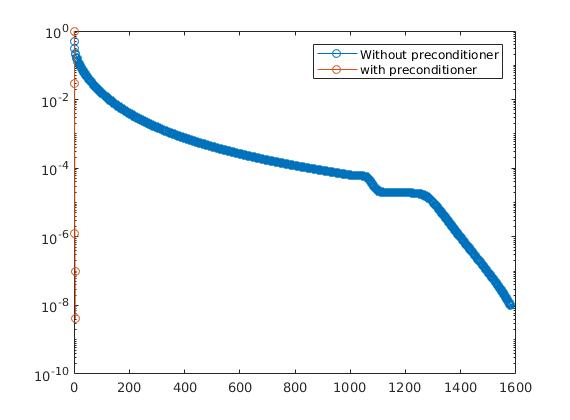
\includegraphics[scale=0.5]{../figs/PrecondNeumannLaplaceSeg.png}
	\caption{Number of iteration in the resolution of the hypersingular  integral equation with a mesh of size $N = 1600$. The importance of preconditioning in this case is more obvious than in the case of the single-layer equation.}
	\label{FigureNitLaplaceNeumann}
\end{figure}

\begin{Rem}
	In \cite{bruno2012second}, the main theorem is equivalent to stating that $N_\omega S_\omega$ and $S_\omega N_\omega$ are bicontinuous operators in $T^s$, with a spectrum concentrated around $\frac{1}{4}$, which can be exploited for preconditioning purposes. It is shown that $N_\omega$ is continuous from $T^s$ to $T^{s-1}$ for all $s >1$ (in fact, this remains true for $s > \frac{1}{2}$). The two main arguments involved in the proof are the explicit expression of $N_\omega T_n$ and the continuity of the adjoint of the Cesaro operator in $l^2(\N)$. The same arguments can be used to prove that $S_\omega$ is also a bicontinuous operator from $U^s$ to $U^{s+1}$ for all $s > 1/2$. 
\end{Rem}



\section{Helmholtz equation}
	
	In this section, we introduce our preconditioners for the Helmholtz integral equations on $\Gamma = (-1,1)$, based on the explicit formulas presented in the previous section. Recall the definition of the single layer and hypersingular operators, $S_k$ and $N_k$, given in \eqref{defSk} and \eqref{defNk}, and the integral equations for the Dirichlet and Neumann problems, \eqref{Sklambda} and \eqref{Nkmu}. As before, let $S_{k,\omega} \isdef S_k \frac{1}{\omega}$ and $N_{k,\omega} \isdef N_k \omega$. The following commutations hold:	
	\begin{The}
		\label{commutations}
		\[S_{k,\omega} \left[-(\omega \partial_x)^2 - k^2\omega^2\right] =  \left[-(\omega \partial_x)^2 - k^2\omega^2\right]S_{k,\omega},\]
		\[N_{k,\omega} \left[-(\partial_x \omega)^2 - k^2\omega^2\right] =  \left[-(\partial_x \omega)^2 - k^2\omega^2\right]N_{k,\omega}.\]
		\begin{proof}
			We start with the first commutation. Since $(\omega \partial_x)^2$ is self adjoint and symmetric, we have 
			\[S_{k,\omega} (\omega \partial_x)^2 = \int_{-1}^{1} \frac{(\omega_y \partial_y)^2 \left[G_k(x-y)\right] u(y)}{\omega(y)},\]
			where we use the notation $\omega_y$ and $\partial_y$ to emphasize the dependence in the variable $y$. 
			Thus, 
			\[S_{k,\omega} (\omega \partial_x)^2 - (\omega \partial_x)^2 S_{k,\omega} = \int_{-1}^{1} \frac{D_k(x,y)u(y)}{\omega(y)},\]
			where $D_k(x,y) \isdef \left[(\omega_y \partial_y)^2 - (\omega_x \partial_x)^2\right] \left[G_k(x-y)\right]$. 
			One has 
			\[D_k(x,y) = G_k''(x-y) (\omega^2_y - \omega^2_x) + G_k'(x-y)(y + x).\]
			Since $G_k$ is a solution of the Helmholtz equation, we have for all $(x \neq y) \in \R^2$ 
			\[G_k'(x-y) = (y-x)(G_k''(x-y) + k^2G(x-y)),\]
			thus
			\[D_k(x,y) = G_k''(x-y)\left(\omega^2_y - \omega_x^2 + y^2 - x^2\right) + k^2(y^2 - x^2)G_k(x-y) . \]
			A careful analysis shows that no Dirac mass appears in the previous formula, that is, the previous formula is an equality of two functions in $T^{-\infty}$. 
			Note that $y^2 - x^2 = \omega_x^2 - \omega_y^2$ so the first term vanishes and we find
			\[S_{k,\omega} (\omega \partial_x)^2 - (\omega \partial_x)^2 S_{k,\omega} =  k^2\left(\omega^2 S_{k,\omega} -S_{k,\omega} \omega^2 \right). \]
			The proof of the second commutation is postponed to \autoref{ann:commut}. 
		\end{proof}
	\end{The}
	
	This theorem implies that the operators $S_{k,\omega}$ and $N_{k,\omega}$ share the same eigenvectors as, respectively, $\left[-(\omega \partial_x)^2 - k^2\omega^2\right]$ and $ \left[-(\partial_x \omega)^2 - k^2\omega^2\right]$. We can look for eigenfunctions of the operator $\left[ -(\omega \partial_x)^2 - k^2\omega^2\right]$, to find a diagonal basis for $S_{k,\omega}$. They are the solutions to the differential equation 
	\[ (1-x^2) y'' - x y' - k^2 \omega^2 y = \lambda y.\]
	Once we set $x = \cos \theta$, $\tilde{y}(\theta) = y(x)$,  $q = \frac{k^2}{4}$, $a = \lambda + 2q$, $\tilde{y}$ is a solution of the standard Mathieu equation 
	\begin{equation}
	\label{MatthieuEq}
		\tilde{y}'' + (a - 2q \cos(2\theta)) \tilde{y} = 0.
	\end{equation}
	There are a discrete set of values $a_{2n}(q)$ for which this equation possesses an even and $2\pi$ periodic function. The corresponding solution is known as the Mathieu cosine, and usually denoted by $\textup{ce}_n$. Here, we use the notation $\textup{ce}^k_n$ to emphasize the dependency in the parameter $k = \sqrt{2q}$ of those functions. The normalization is taken as
	\[ \int_{0}^{2\pi} \textup{ce}^k_n(\theta)^2 d\theta = \pi.\]
 	The Matthieu cosines also satisfy
	\[ \int_{-\pi}^{\pi}\textup{ce}^k_n(\theta) \textup{ce}^k_m(\theta) = \pi \delta_{m,n}.\]
	so that any even $2\pi$ periodic function in $L^2(-\pi,\pi)$ can be expanded along the functions $\textup{ce}_n$, with the coefficients obtained by orthonormal projection. Letting 
	\[T_{n}^k \isdef \textup{ce}^k_n(\arccos(x)),\]
	in analogy to the zero-frequency case, we have
	\[\left[-(\omega \partial_x)^2 - k^2\omega^2\right] T_{n}^k = \lambda_{n,k}^2 T_{n}^k.\]
	For large $n$, using the general results from the theory of Hill's equations (see \cite[eq. 28.29.21]{NIST:DLMF}) we have the following asymptotic formula for $\lambda_{n,k}$:
	\[ \lambda_{n,k}^2 = n^2 - \frac{k^4}{16n^2} +o \left(n^{-2}\right). \]
	The first commutation established in \autoref{commutations} implies that the Matthieu cosines are also the eigenfunctions of the single-layer operator. An equivalent statement is given in \cite[Thm 4.2]{betcke2014spectral}, if we allow the degenerate case $\mu = 0$. 
	
	A similar analysis can be applied to the hypersingular operator. The eigenfunctions of $\left[(\partial_x \omega)^2 - k^2 \omega^2\right]$ are given by 
	\[U_n^k \isdef \frac{\textup{se}_n^k(\arccos(x))}{\omega(x)}\]
	where $\textup{se}_n^k$ are the so-called Matthieu sines, which also satisfy the Matthieu differential equation \eqref{MatthieuEq}, but with the condition that they must be odd $2\pi$ periodic functions. 
	
	All the previous considerations highly suggest that the following theorem should hold:	
	\begin{The} 
		There exists a compact operator $K$ from $T^s$ to $T^{s+2}$ such that
		\[\left[-(\omega \partial_x)^2 - k^2\omega^2\right]S_{k,\omega}^2 = \frac{I_d}{4} + K, \]
		and a compact operator $K'$ from $U^s$ to $U^{s-2}$ such that
		\[N_{k,\omega}^2 = \left[-(\partial_x \omega)^2 - k^2 \omega^2\right] + K'.\]
	\end{The}
The proof of this theorem, however, requires the introduction of additional analytic tools. In order to keep a concise presentation, it is thus omitted in the present work. Full details can be found in \cite{}. As a consequence, the operator $\left[-(\omega \partial_x)^2 - k^2 \omega^2\right]^{1/2}$ should be a good preconditioner for $S_{k,\omega}$, as well as $\left[-(\partial_x \omega)^2 - k^2 \omega^2\right]^{-1/2}$ for $N_{k,\omega}$. 
In the more general case of a $C^{\infty}$ non-intersecting open curve $\Gamma$ and non-zero frequency $k$, the previous result extends, replacing $\omega$ by $\omega_\Gamma(x) = \abs{\Gamma} \omega(x)$, where $\abs{\Gamma}$ is the length of the curve, $\partial_x$ by $\partial_\tau$ the tangential derivative on $\Gamma$ and $S_{k,\omega_{\Gamma}} \isdef S_k \frac{1}{\omega_\Gamma}$, $N_{k,\omega_{\Gamma}} \isdef N_k \omega_\Gamma$. 

\section{Numerical results}
\label{sec:NumericalResutls}

In this section, we show some numerical results to illustrate the efficiency of the introduced preconditioners for the Helmholtz equation. Numerical tests are run with a high-level programming language, on a 16GB RAM laptop, \toDo{Spec de l'ordis à terminer}. Numerical methods are detailed in \autoref{sec:numerMeth}. In each case, to fully resolve the frequency, the number of segments in the discretization is set to $N \approx 10k$, where $k = \frac{\pi}{\lambda}$ is the wavenumber. In the GMRES iteration, we require a relative residual below $1e-8$. 
\paragraph{Flat segment, Dirichlet boundary condition.} In \autoref{TableNitTimeHlemholtzDirichlet} we report the number of GMRES iterations for the numerical resolution of Equation \eqref{Somegaalpha} on the segment $\Gamma = (-1,1)$, when the linear system is preconditioned by the operator $\sqrt{-(\omega \partial_x)^2 - k^2 \omega^2}$, as compared to the case where no preconditioner is used.  In \autoref{FigureNitHelmDirichlet}, we plot the relative residual history in the GMRES method with and without preconditioner for a problem with $L = 400 \lambda$. The Dirichlet data is set to $u_D(x) = e^{ikx}$. 
\begin{table}[H]
	\begin{center}
		\begin{tabular}{|| m{4em} | m{4em} | m{4em} | m{4em} | m{4em}||} 
			\hline
			\multicolumn{1}{||c|}{ }&
			\multicolumn{2}{c|}{with Prec.}&\multicolumn{2}{c||}{without Prec.}\\
			\hline
			$L/\lambda$ & $n_{it}$& t(s) & $n_{it}$ & t(s)\\
			\hline\hline
			50 & 8 & 0.1 & 73 & 0.28\\
			\hline
			200 & 10 & 1.3 & 116 & 17\\
			\hline
			800 & 15 & 34 & 148 & 300\\
			\hline
		\end{tabular}
	\end{center}
	\caption{Number of iteration and time needed for the numerical resolution of \eqref{Somegaalpha} using Galerkin finite elements with and without preconditioner.}
	\label{TableNitTimeHlemholtzDirichlet}
\end{table}
\vspace{-1cm}
\begin{figure}[H]
	\centering
	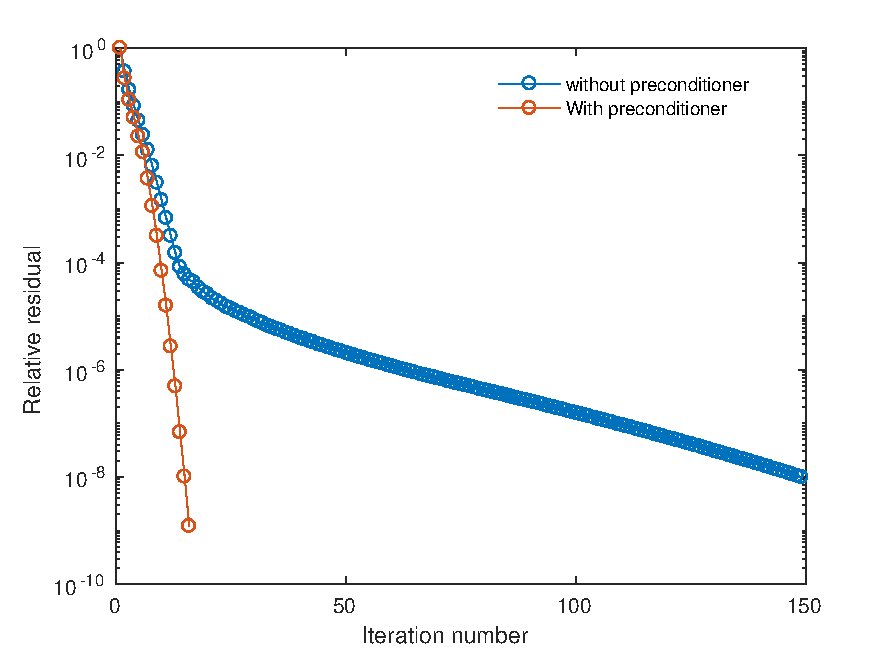
\includegraphics[scale=0.5]{../figs/PrecondDirichletHelmSegPDF}
	\caption{Number of iteration in the resolution of the single layer integral equation with a mesh of size $N \approx 3700$, $L = 800 \lambda$.}
	\label{FigureNitHelmDirichlet}
\end{figure}
\paragraph{Flat segment, Neumann boundary condition.} We run the same numerical comparisons, this time with the precondioning operator $\left(-(\partial_x \omega)^2 - k^2 \omega^2\right)^{-1/2}$. 
\begin{table}[H]
	\begin{center}
		\begin{tabular}{|| m{4em} | m{4em} | m{4em} | m{4em} | m{4em}||} 
			\hline
			\multicolumn{1}{||c|}{ }&
			\multicolumn{2}{c|}{with Prec.}&\multicolumn{2}{c||}{without Prec.}\\
			\hline
			$L/\lambda$ & $n_{it}$& t(s) & $n_{it}$ & t(s)\\
			\hline\hline
			50 & 8 & 0.08 & 785 & 9.4\\
			\hline
			200 & 10 & 3.6 & - &  $>$ 2min\\
			\hline
			800 & 17 & 73 & - & -\\
			\hline
		\end{tabular}
	\end{center}
	\caption{Number of iteration and time needed for the numerical resolution of \eqref{Somegaalpha} using Galerkin finite elements with and without preconditioner.}
	\label{TableNitTimeHlemholtzNeumann}
\end{table}
\vspace{-1cm}
\begin{figure}[H]
	\centering
	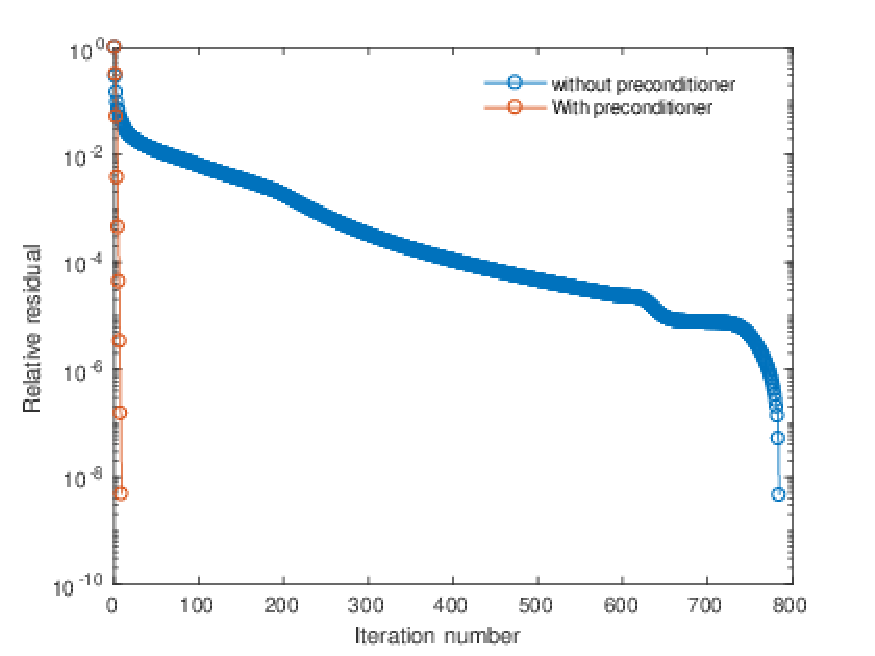
\includegraphics[scale=0.5]{../figs/PrecondNeumannHelmSegPDF}
	\caption{Number of iteration in the resolution of Hypersingular integral equation with a mesh of size $N \approx 800$, $L = 50 \lambda$.}
	\label{FigureNitHelmNeumann}
\end{figure}
\paragraph{Non-flat arc.} Here, we also report numerical results when the curve is a portion of spiral (see \autoref{ArcOfSpiral}), for both boundary conditions. This shows that the preconditioning strategy is also efficient in presence of non-zero curvature. 
\begin{table}[H]
	\begin{center}
		\begin{tabular}{|| m{4em} | m{4em} | m{4em} | m{4em} | m{4em}||} 
			\hline
			\multicolumn{1}{||c|}{ }&
			\multicolumn{2}{c|}{Dirichlet}&\multicolumn{2}{c||}{Neumann}\\
			\hline
			$L/\lambda$ & $n_{it}$& t(s) & $n_{it}$ & t(s)\\
			\hline\hline
			50 & 23 & 0.6 & 785 & 9.4\\
			\hline
			200 & 27 & 9 & - &  $>$ 2min\\
			\hline
			800 & 40 & 35 & - & -\\
			\hline
		\end{tabular}
	\end{center}
	\caption{Number of iterations of the preconditioned system. \toDo{Itérations et temps à remplir pour Neumann}}
	\label{TableNitTimeHlemholtzDirSpiral}
\end{table}
\vspace{-1cm}
\begin{figure}[H]
	\centering
	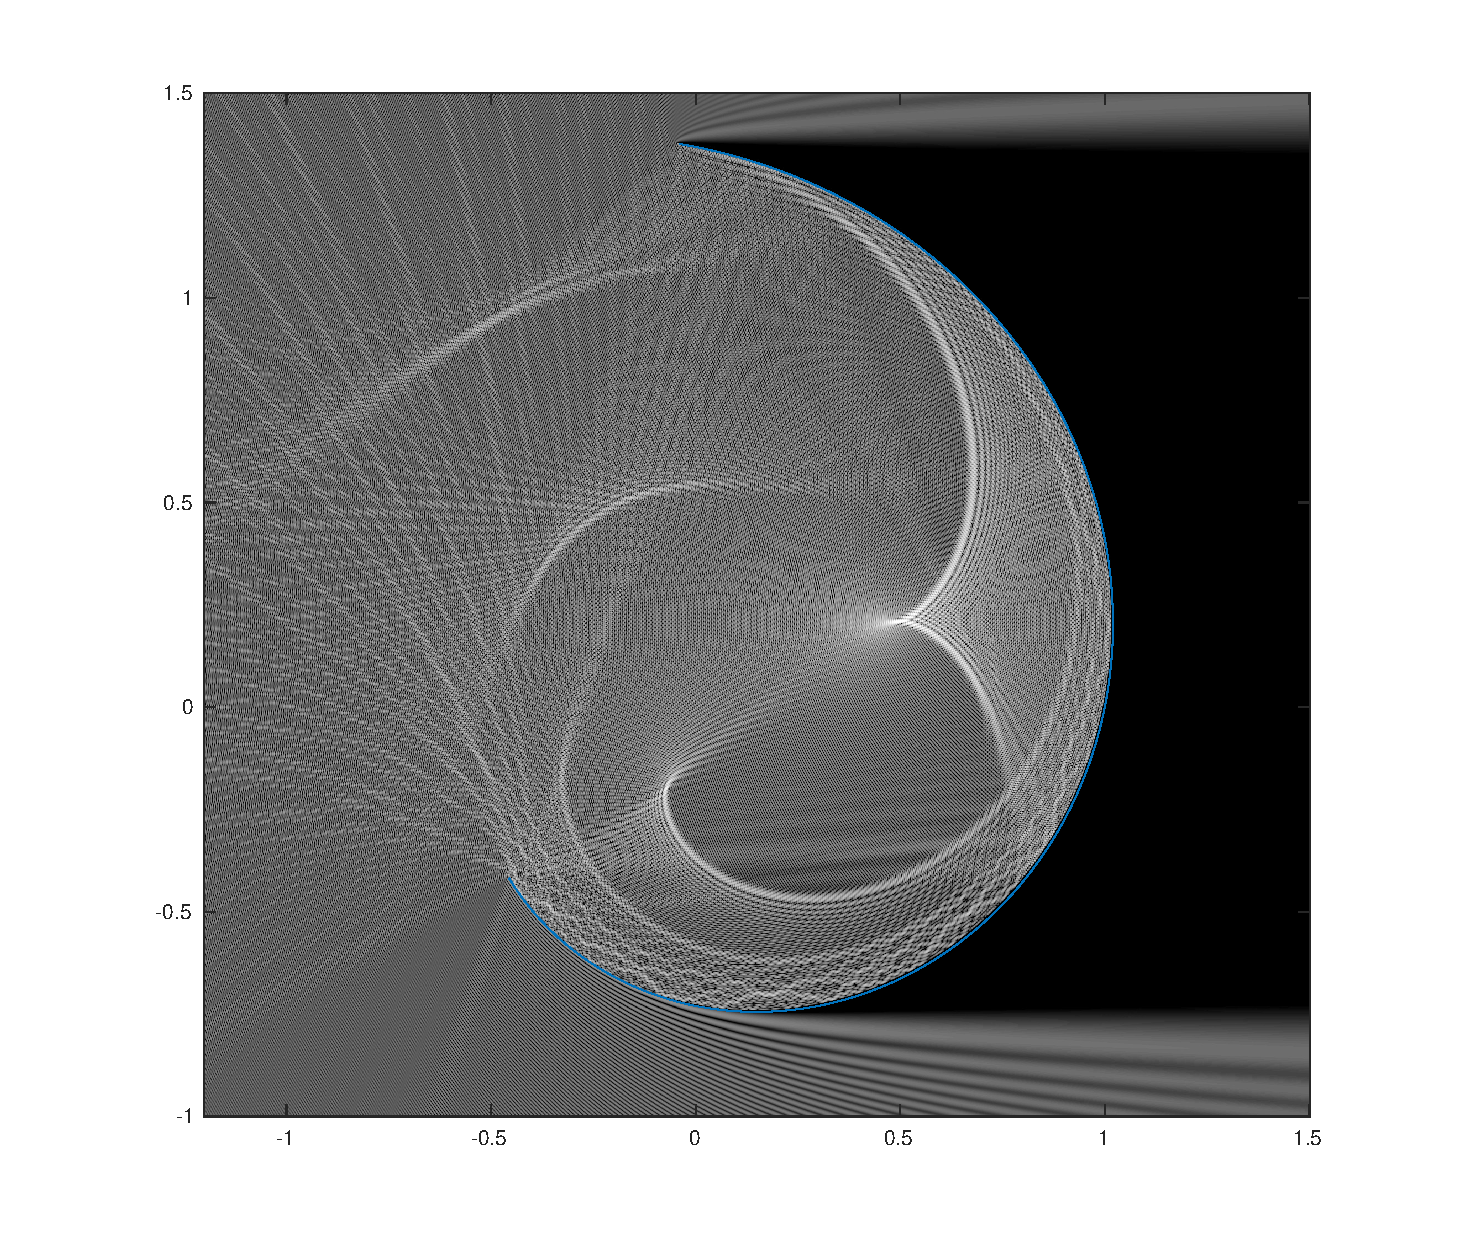
\includegraphics[width=\linewidth]{../figs/arcOfSpiral800_3}
	\vspace{-1.2cm}
	\caption{Sample diffraction pattern (Dirichlet boundary conditions) with left to right incidence for an arc of spiral of size $L = 800 \lambda$. After the resolution of the integral equation, the image is obtained in a few seconds.}
	\label{ArcOfSpiral}
\end{figure}
\paragraph{Comparison with the generalized Calderon relations.} As shown in \cite{bruno2012second}, $S_\omega$ and $N_\omega$ can be used efficiently as mutual preconditioners. This alternative method is also very efficient in our numerical setting (here, we use simple piecewise affine functions, whereas in \cite{bruno2012second}, spectral discretization with trigonometric polynomials is used). We report in \autoref{TableBrunoVsSqrt} the number of iterations and computing times for the Neumann problem with an angle of incidence $\frac{\pi}{4}$ on the flat segment. The number of iterations is comparable for the two methods. However, the matrix-vector product time in our method is significantly slower as it only involves sparse operators. This leads to a faster resolution of the linear system. 

\begin{table}[H]
	\begin{center}
		\begin{tabular}{|| m{4em} | m{4em} | m{4em} | m{4em} | m{4em}||} 
			\hline
			\multicolumn{1}{||c|}{ }&
			\multicolumn{2}{c|}{Calderon Prec.}&\multicolumn{2}{c||}{Square root Prec.}\\
			\hline
			$L/\lambda$ & $n_{it}$& t(s) & $n_{it}$ & t(s)\\
			\hline\hline
			50 & 14 & 0.1 & 8 & 0.1\\
			\hline
			200 & 15 & 7.5 & 11 &  3.6\\
			\hline
			800 & 16 & 130 & 15 & 70\\
			\hline
		\end{tabular}
	\end{center}
	\caption{Number of iteration and time needed for the numerical resolution of \eqref{Somegaalpha} using Galerkin finite elements with and without preconditioner.}
	\label{TableBrunoVsSqrt}
\end{table}
	
\section{Numerical methods}
\label{sec:numerMeth}
	
	\toDo{J'ai commencé mais c'est sur l'autre ordi. À inclure}.
	
\section{Conclu} 
	
\appendix
\section{Commutation of $N_\omega$ and $(\partial_x \omega)^2 + k^2\omega^2$}
\label{ann:commut}
\begin{Lem}
	\label{dxSomega2=Somegadxomega}
	For any $\phi$, there holds 
	\[\partial_x S_\omega \omega^2 \phi = S_\omega \omega \partial_x \omega \phi.\]
\end{Lem}
\begin{proof}
	In our context, the largest space encountered is $U^{- \infty}$ (As a consequence of \autoref{inclusionsTsUs}) so we shall show that this identity holds in that space.
	For any $s$, $\omega^2$ is a continuous operator from $U^s$ to $T^s$, $S_\omega$ is continuous from $T^s$ to $T^{s+1}$ and $\partial_x$ is continuous from $T^{s+1}$ to $U^s$. Indeed, we have 
	\[\omega^2 U_n = \frac{T_n - T_{n+2}}{2}\] 
	and 
	\[\partial_x T_n = n U_{n-1}.\]
	Therefore, the left operator is continuous from $U^s$ to $U^s$. Similarly, the right operator is continuous from $U^{s}$ to $U^s$ for all $s$. If we fix $\phi \in U^{s}$ for some $s$, using the decomposition of $\phi$ on $U_n$, there exists a sequence $\phi_N$ in $U^{\infty}$ converging to $\phi$ in $U^{s}$. It is thus sufficient to check the identity for $\phi = U_n$. For $n \geq 1$, 
	\begin{eqnarray*}
		\partial_x S_\omega \omega^2 U_n &=& \partial_x S_\omega \left(\frac{T_{n} - T_{n+2}}{2}\right)\\
		&=& \partial_x\left(\frac{T_{n}}{4n} - \frac{T_{n+2}}{4(n+2)} \right)\\
		&=& \frac{U_{n-1} - U_{n+1}}{4}\\
		&=& -\frac{T_{n+1}}{2}.
	\end{eqnarray*}
	One can check that the result also holds for $n = 0$. On the other hand, for all $n$, 
	\begin{eqnarray*}
		S_\omega \omega \partial_x \omega U_n &=&-(n+1) S_\omega T_{n+1}\\
		&=& -\frac{1}{2}T_{n+1}
	\end{eqnarray*}
	which proves the result. 
\end{proof}
We now turn to the proof of the theorem. To ease the computations, we take some notations: let $\Delta_\omega \isdef (\omega \partial_x)^2$, $\Delta_\omega^T \isdef (\partial_x \omega)^2$,  $N_\omega \isdef N_{k,\omega}$, and $S_\omega \isdef S_{k,\omega}$. Using, equation \eqref{NkenfonctiondeSk} we can write 
\[N_\omega = -\partial_x S_\omega \omega \partial_x \omega - k^2 S_\omega \omega^2.\]
To show that $N_\omega$ and $\Delta_\omega^T + k^2\omega^2$ commute, we compute their commutator $C$ and show that it is null. 
We have 
\begin{eqnarray*}
	C &\isdef& N_\omega \Delta_\omega^T - \Delta_\omega^T N_\omega + k^2N_\omega \omega^2 - k^2 \omega^2 N_\omega \\
	&=& -\partial_x S_\omega \Delta_\omega \omega \partial_x \omega  - k^2 S_\omega \omega^2 \Delta_\omega^T \\
	&& + \partial_x \Delta_\omega S_\omega \omega \partial_x \omega + k^2 \Delta_\omega^T S_\omega \omega^2 \\
	&& - k^2 \partial_x S_\omega \omega \partial_x \omega^3 - k^4 S_\omega \omega^4 \\
	&& + k^2 \omega^2 \partial_x S_\omega \omega \partial_x \omega + k^4 \omega^2 S_\omega \omega^2
\end{eqnarray*}
where each term in the r.h.s. of the first equality gives rise to a line in the second. We rearrange the terms as follows:
\begin{eqnarray*}
	C &=& \partial_x (\Delta_\omega S_\omega - S_\omega \Delta_\omega) \omega \partial_x \omega - k^2 \partial_x S_\omega \omega \partial_x \omega^3 + k^2 \omega^2 \partial_x S_\omega \omega\partial_x \omega\\	
	&& + k^4 (\omega^2 S_\omega - S_\omega \omega^2) \omega^2\\
	&& + k^2(\Delta_\omega^T S_\omega \omega^2 - S_\omega \omega^2 \Delta_\omega^T)
\end{eqnarray*}
For the first term, we inject the commutation shown in \autoref{commutations}. For the last line, we use the following identities: 
\[ \Delta_\omega^T = \Delta_\omega - 2x \partial_x - 1\]
\[ \omega^2 \Delta_\omega^T = \Delta_\omega \omega^2 + \omega^2 + 2 \omega x \partial_x \omega\]
Let $D = \frac{C}{k^2}$, 
\begin{eqnarray*}
	D &=& \partial_x S_\omega \omega (\omega^2\partial_x - \partial_x \omega^2) \omega  + (\omega^2 \partial_x - \partial_x \omega^2)S_\omega \omega \partial_x \omega\\
	&&+ k^2(\omega^2 S_\omega - S_\omega \omega^2) \omega^2\\
	&&+ (\Delta_\omega - 2x \partial_x - 1)S_\omega \omega^2 - S_\omega(\Delta_\omega \omega^2 + \omega^2 + 2\omega x \partial_x \omega) 
\end{eqnarray*}
We use $\omega^2 \partial_x - \partial_x \omega^2 = 2x$, and the relation $\partial_x S \omega^2 = S_\omega \omega \partial_x \omega$ to get
\begin{eqnarray*}
	D &=& 2 S_\omega \omega \partial_x x\omega + 2 x S_\omega  \omega \partial_x \omega \\
	&& + \left(k^2(\omega^2 S_\omega - S_\omega \omega^2) + \Delta_\omega S_\omega - S_\omega \Delta_\omega \right)\omega^2\\
	&& - 2 S_\omega \omega^2 - 2 x  S_\omega \omega \partial_x \omega - 2 S_\omega \omega x \partial_x \omega.
\end{eqnarray*}
Using again the commutation shown in \autoref{commutations}, we are left with 
\begin{eqnarray*}
	D &=&  2 S_\omega \omega (\partial_x x - x \partial_x) \omega - 2 S_\omega \omega^2
\end{eqnarray*}
This is null since $\partial_x x - x \partial_x = 1$. 

	
	
	
	
	
	\bibliographystyle{plain}
	\IfFileExists{biblio.bib}{\bibliography{biblio}}{\bibliography{../../Biblio/biblio}}
	
	
\end{document}


